%%%%%%%%%%%%%%%%%%%%%%%%%%%%%%%%%%%%%%%%%%%%%%%%%%%%%%%%%%%%%%%%%%%%%%%%%%%%%%%%%%
\begin{frame}[fragile]\frametitle{}
\begin{center}
{\Large Conclusion}
\end{center}
\end{frame}

%%%%%%%%%%%%%%%%%%%%%%%%%%%%%%%%%%%%%%%%%%%%%%%%%%%
\begin{frame}[fragile]\frametitle{What did you learn?}
\begin{center}
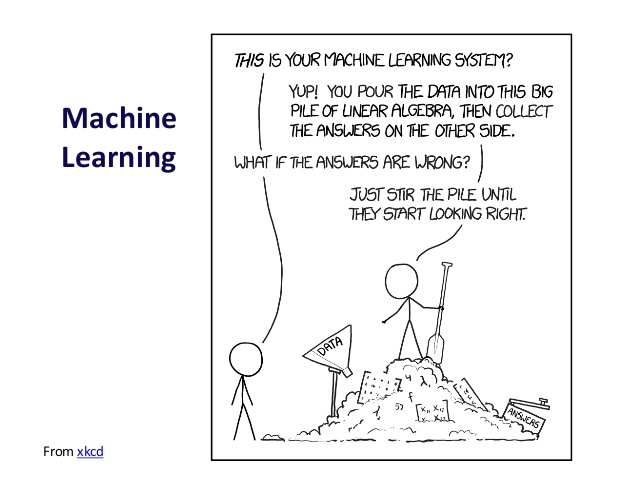
\includegraphics[width=0.8\linewidth,keepaspectratio]{xkcdml}
\end{center}
\end{frame}

%%%%%%%%%%%%%%%%%%%%%%%%%%%%%%%%%%%%%%%%%%%%%%%%%%%%%%%%%%%%%%%%%%%%%%%%%%%%%%%%%%
\begin{frame}[fragile]\frametitle{}
\begin{center}
{\Large ML Recap}

{\tiny (Ref: ``Machine Learning Algorithm Cheat Sheet'' - Laura Diane Hamilton)}
\end{center}
\end{frame}

%%%%%%%%%%%%%%%%%%%%%%%%%%%%%%%%%%%%%%%%%%%%%%%%%%%%%%%%%%%%%%%%%%%%%%%%%%%%%%%%%%
\begin{frame}\frametitle{Linear regression}
Theme: Fitting Line

   \begin{columns}[t]
    \begin{column}{0.3\linewidth}
	\textbf{Pros}
		\begin{itemize}
		\item Very fast (runs in constant time)
		\item Easy to understand the model
		\item  Less prone to over-fitting
		\end{itemize}
    \end{column}
    \begin{column}{0.3\linewidth}
	\textbf{Cons}
			\begin{itemize}
		\item  Unable to model complex relationships
		\item Unable to capture nonlinear relationships without first
transforming the inputs
		\end{itemize}
    \end{column}
	
    \begin{column}{0.3\linewidth}
	\textbf{Good at}
			\begin{itemize}
		\item  The first look at a dataset
		\item  Numerical data with lots of features
		\end{itemize}
    \end{column}
	
  \end{columns}
\end{frame}


%%%%%%%%%%%%%%%%%%%%%%%%%%%%%%%%%%%%%%%%%%%%%%%%%%%%%%%%%%%%%%%%%%%%%%%%%%%%%%%%%%
\begin{frame}\frametitle{Decision trees}
Theme: Fitting a tree

   \begin{columns}[t]
    \begin{column}{0.3\linewidth}
	\textbf{Pros}
		\begin{itemize}
		\item Fast
		\item Robust to noise and missing values
		\item Accurate
		\end{itemize}
    \end{column}
    \begin{column}{0.3\linewidth}
	\textbf{Cons}
			\begin{itemize}
		\item   Complex trees are hard to interpret
		\item Duplication within the same sub-tree is possible
		\end{itemize}
    \end{column}
	
    \begin{column}{0.3\linewidth}
	\textbf{Good at}
			\begin{itemize}
		\item   Medical diagnosis
		\item  Credit risk analysis
		\end{itemize}
    \end{column}
	
  \end{columns}
\end{frame}



%%%%%%%%%%%%%%%%%%%%%%%%%%%%%%%%%%%%%%%%%%%%%%%%%%%%%%%%%%%%%%%%%%%%%%%%%%%%%%%%%%
\begin{frame}\frametitle{Support Vector
Machines}
Theme: Partitioning Hyperplanes with wide margins

   \begin{columns}[t]
    \begin{column}{0.3\linewidth}
	\textbf{Pros}
		\begin{itemize}
		\item  Can model complex, nonlinear relationships
		\item Robust to noise (because they maximize
margins)
		\end{itemize}
    \end{column}
    \begin{column}{0.3\linewidth}
	\textbf{Cons}
			\begin{itemize}
		\item   Need to select a good kernel function
		\item  Model parameters are difficult to interpret
		\end{itemize}
    \end{column}
	
    \begin{column}{0.3\linewidth}
	\textbf{Good at}
			\begin{itemize}
		\item   Handwriting recognition
		\item  Text classification
		\end{itemize}
    \end{column}
	
  \end{columns}
\end{frame}


%%%%%%%%%%%%%%%%%%%%%%%%%%%%%%%%%%%%%%%%%%%%%%%%%%%%%%%%%%%%%%%%%%%%%%%%%%%%%%%%%%
\begin{frame}\frametitle{K-Nearest Neighbors}
Theme: Partitioning Hyperplanes with wide margins

   \begin{columns}[t]
    \begin{column}{0.3\linewidth}
	\textbf{Pros}
		\begin{itemize}
		\item   Simple, Powerful
		\item  No training involved (``lazy'')
		\item Naturally handles multiclass classification
and regression
		\end{itemize}
    \end{column}
    \begin{column}{0.3\linewidth}
	\textbf{Cons}
			\begin{itemize}
		\item   Expensive and slow to predict new instances
		\item  Performs poorly on high-dimensionality datasets
		\item   Must define a meaningful distance function
		\end{itemize}
    \end{column}
	
    \begin{column}{0.3\linewidth}
	\textbf{Good at}
			\begin{itemize}
		\item  Low-dimensional datasets
		\item  Fault detection 
		\end{itemize}
    \end{column}
	
  \end{columns}
\end{frame}



%%%%%%%%%%%%%%%%%%%%%%%%%%%%%%%%%%%%%%%%%%%%%%%%%%%%%%%%%%
\begin{frame}[fragile]\frametitle{Comparing ML Algorithms}
\begin{itemize}
\item  Power and Expressibility: ML methods differ in terms
of complexity. Linear regression fits linear functions while NN define piecewise-linear separation boundaries. More complex models can provide more accurate models, but
at the risk of over-fitting.
\item  Interpret-ability: some models are more transparent
and understandable than others (white box vs. black box
models)
\item  Ease of Use: some models feature few parameters/decisions (linear regression/NN), while others
require more decision making to optimize (SVMs)
\item  Training Speed: models differ in how fast they fit the
necessary parameters
\item  Prediction Speed: models differ in how fast they make
predictions given a query
\end{itemize}
(pto \ldots)
\end{frame}


%%%%%%%%%%%%%%%%%%%%%%%%%%%%%%%%%%%%%%%%%%%%%%%%%%%%%%%%%%
\begin{frame}[fragile]\frametitle{KNN Regression Example: 1d}
\begin{center}
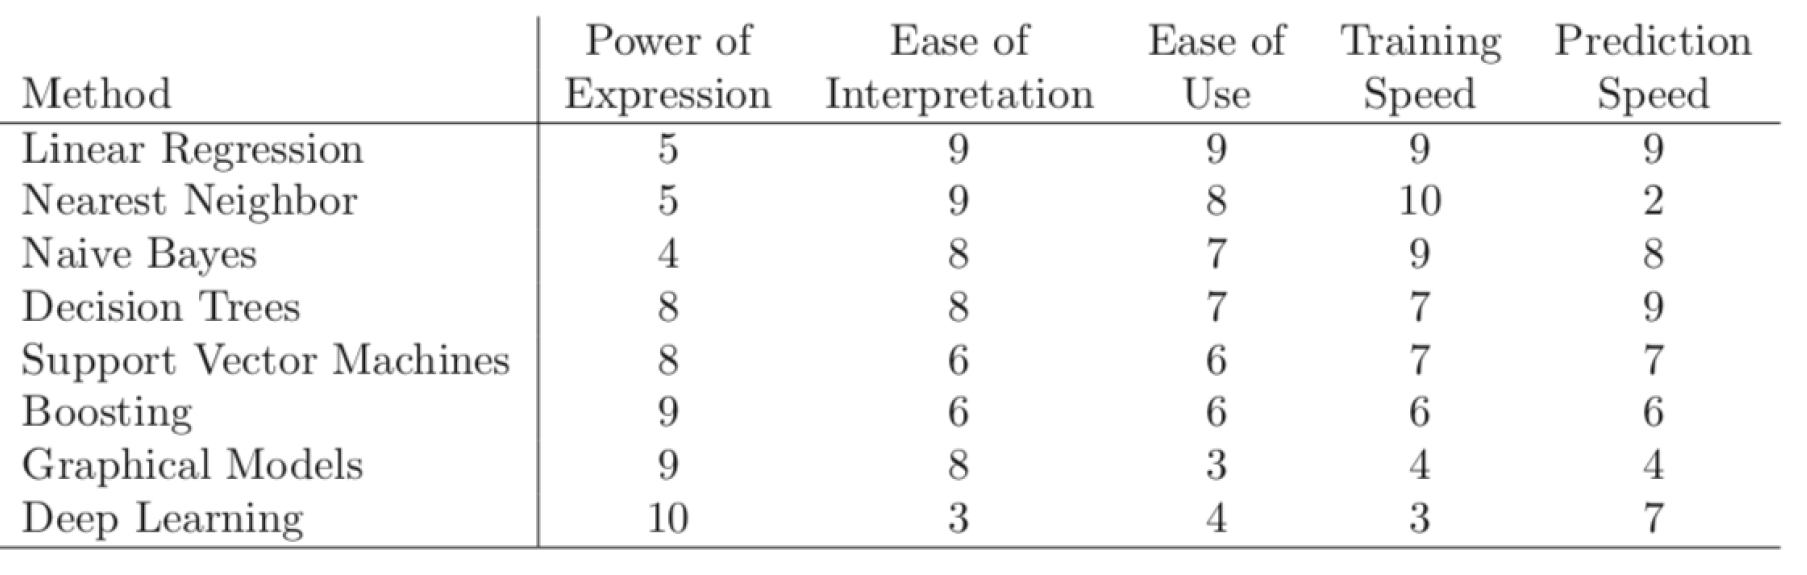
\includegraphics[width=\linewidth,keepaspectratio]{mlall}
\end{center}
\end{frame}

%%%%%%%%%%%%%%%%%%%%%%%%%%%%%%%%%%%%%%%%%%%%%%%%%%%%%%%%%%%%%%%%%%%%%%%%%%%%%%%%%%
\begin{frame}[fragile]\frametitle{}
\begin{center}
{\Large What Next?}
\end{center}
\end{frame}

%%%%%%%%%%%%%%%%%%%%%%%%%%%%%%%%%%%%%%%%%%%%%%%%%%%%%%%%%%%%%%%%%%%%%%%%%%%%%%%%%%
\begin{frame}\frametitle{Machine Learning Journey}
To start with \ldots

\footnotesize
\begin{itemize}
\item If you want a more practical route then: Udacity Intro to Machine Learning
\item If you want to learn Machine Learning in-depth then: Coursera Machine Learning Andrew Ng
\item  If you want other free courses, blogs, and books then: Phoenixts
\item  After being familiar with that, you should try learning:
\begin{itemize}
\item  How to Approach Almost Any ML Problem - Abhishek Thakur
\item  Bias Variance Trade-Off
http://scott.fortmann-roe.com/docs/BiasVariance.html
\item  Measuring Errors
http://scott.fortmann-roe.com/docs/MeasuringError.html
\item  ROC Curve \& AUC Explained
https://www.youtube.com/watch?v=OAl6eAyP-yo
\end{itemize}
\end{itemize}

(Ref: ``Simple 8 Step guide to learn Machine Learning with Python'' - Randy Lao)
\end{frame}

%%%%%%%%%%%%%%%%%%%%%%%%%%%%%%%%%%%%%%%%%%%%%%%%%%%%%%%%%%%%%%%%%%%%%%%%%%%%%%%%%%%%%%%%%%%%%%%%%%%%%%%%%%%%%%%%%%%%%%%%%
\begin{frame}\frametitle{Machine Learning Learning Path}
After you are done with Python \ldots

\footnotesize
\begin{itemize}
\item Machine Learning in 20min: https://www.youtube.com/watch?v=MOdlp1d0PNA
\item Skcikit-Learn Tutorial: https://www.youtube.com/watch?v=elojMnjn4kk
\item Kaggle Machine Learning Tutorial: https://www.kaggle.com/learn/machine-learning
\item Google Crash coursr Machine Learning 
\item Machine Learning at Berkeley
https://ml.berkeley.edu/blog/tutorials/
\item How to Learn Machine Learning in 6 Months
https://www.youtube.com/watch?v=MOdlp1d0PNA\&t=584s
\item Learning Machine Learning \& AI Guideline
https://www.youtube.com/watch?v=PYKfXkd3t7c

\item edX – Machine Learning (Columbia University, John Paisley)
https://www.edx.org/course/machine-learning-columbiax-csmm-102x-0
\item sentdex – Practical Machine Learning Tutorial (Youtube)
\end{itemize}

(Ref: ``To start your DataScience Journey'' - Randy Lao)
\end{frame}


%%%%%%%%%%%%%%%%%%%%%%%%%%%%%%%%%%%%%%%%%%%%%%%%%%%%%%%%%%%%%%%%%%%%%%%%%%%%%%%%%%%%%%%%%%%%%%%%%%%%%%%%%%%%%%%%%%%%%%%%%
\begin{frame}\frametitle{Transitioning into DataScience}
Some amazing advice for those transitioning into DataScience: \ldots

\footnotesize
\begin{itemize}
\item Kyle McKiou - DS Interview
\item Sarah Nooravi - Personal Skills
\item Beau Walker - How to Gain Experience
\item Eric Weber - DS Companies
\item Vin Vashishta - DS Interviews \& Your Persona
\item Kevin Tran - How to Land Your 1st DS Job
\item David Langer - The 80/20 Rule of DS
\item Favio Vázquez - Persistence 
\item Nic Ryan - Your Game Plan
\end{itemize}

(Ref: ``Transitioning into DataScience'' - Randy Lao)
\end{frame}

